\documentclass[a4paper,12pt]{article} % Класс документа

% Подключаем полезные пакеты
\usepackage{booktabs}  % для \toprule, \midrule, \bottomrule
\usepackage{caption}   % улучшает внешний вид подписей
\usepackage{geometry}  % необязательно, просто удобнее
\geometry{margin=2cm}
\usepackage[utf8]{inputenc}    % Кодировка UTF-8
\usepackage[T2A]{fontenc}      % Кириллица
\usepackage[russian]{babel}    % Русский язык
\usepackage{amsmath, amssymb}  % Математика
\usepackage{graphicx}          % Для вставки изображений
\usepackage{hyperref}          % Ссылки и кликабельные URL
\usepackage{geometry}          % Настройка полей

\usepackage{titlesec}

\titleclass{\subsubsubsection}{straight}[\subsubsection]

\newcounter{subsubsubsection}[subsubsection]
\renewcommand\thesubsubsubsection{\thesubsubsection.\arabic{subsubsubsection}}

\titleformat{\subsubsubsection}
  {\normalfont\normalsize\bfseries}
  {\thesubsubsubsection}{1em}{}

\titlespacing*{\subsubsubsection}{0pt}{3.25ex plus 1ex}{1.5ex plus .2ex}

\setcounter{secnumdepth}{4}
\setcounter{tocdepth}{4}

\title{Ультразвуковая локальная навигация}
\author{Смирнов Егор Ильич}
\date{}

\begin{document}

\maketitle % Заголовок статьи

\subsection{Задача}

Необходимо реализовать систему локальной навигации для БПЛА на подвижной платформе.
\section{Теория}

\subsection{Принцип работы}


Известная скорость звука в середе позволяет измерять расстоние, путем замера времени прохождения сигнала.
Таким образом можно выяснить расстояние между излучателем и приемником, при условии синхронных часов на них.

Идея состоит в размещении трех и более приемников (или излучателей) в разных местах с известными координатами. Подвижный обьект будет нести на себе излучатель (или приемник). Далее измеряется расстояние от обьекта до опорных точек и, решая систему уравнений, можно вычислить координаты обьекта.

\subsection{Физика}
Разберемся с физикой процессов и физическими ограничениями.
\subsubsection{Скорость звука}
Для рассмотрения скорости звука достаточно приближения идеального газа. Классическая формула выглядит так:
\begin{equation}
c = \sqrt{\frac{\gamma R T}{M}}
\end{equation}
где:
\begin{itemize}
\item $\gamma$ — показатель адиабаты (для воздуха $\approx$ 1.4),
\item R — универсальная газовая постоянная R=8.314 Дж/(моль $\cdot$ К)
\item T — абсолютная температура, К,
\item M — молярная масса воздуха ($\approx$ 0.02896 кг/моль).
\end{itemize}
Таким образом на скорость распространения звука может повлиять температура и влажность воздуха (влажность влияет на среднюю молярную массу среды).

\begin{equation}
c = 331.4 + 0.6t + 0.0124H
\end{equation}
где $H$ — относительная влажность в процентах.
\subsubsection{Затухание амплитуды звука}
С затуханием разобраться немного сложнее.

Интенсивность звука убывает с расстоянием как:
\begin{equation}
 I(x) = I_0e^{-\alpha x}
\end{equation}
$\alpha$ - коэфицент затухания

\vspace{5mm}
Для коэфицента затухания формула очень сложная, приводить ее здесь не вижу смысла.

В python были произведены расчеты затухания звукового сигнала с помощью формулы ISO-9613-1


\begin{figure}[h!]
    \centering
    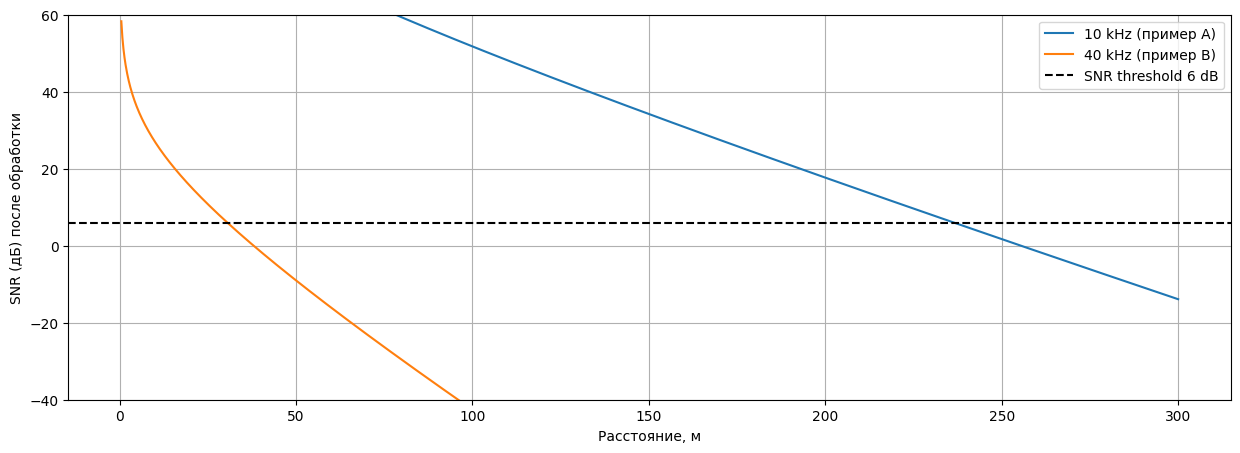
\includegraphics[width=1\textwidth]{output.png} % замените на свой файл
    \caption{график затухания звукового сигнала}
    \label{fig:example}
\end{figure}

Эти расчеты позволяют оценить примерное максимальное расстояние между излучателем и приемником.

\vspace{5mm}

(10 kHz): alpha = 0.2806 dB/m, max range (SNR>=6 dB) = 236.3 m

(40 kHz): alpha = 0.5515 dB/m, max range (SNR>=6 dB) = 25.8 m

\vspace{5mm}
расчеты производились при следующих параметрах:
\begin{itemize}
\item относительная влажность - 50%
\item температура воздуха - 20 C
\item мощность УК излучателя - 105 dB (SPL 1m)
\item чувствительность УК приемника - -95 dB
\end{itemize}

В расчетах видно, что звук высокой частоты затухает значительно сильнее чем низкой. Однако в коммерчиских системах чаще выберают именно ультразвук так как он не является слышимым (что однозначто плюс) и лучше отражается от различных поверхностей (важно для дальномеров). Также в ультрахзвуке меньше внешнего шума.

\subsubsection{Точность измерений}
В ToF (Time of Flight) варианте, ключевую роль играет дискретность измерений по времени $\Delta t$. 

Ошибка измерений расстояния будет соответсвенно:
\begin{equation}
 \pm d = \frac{c}{2 \Delta t}
\end{equation}

Приведем характерные значения:

\begin{table}[h!]
    \centering
    \begin{tabular}{|c|c|}
        \hline
        $\Delta t$ & $d$ \\
        \hline
        1 мкс & 0.17 мм  \\
        10 мкс & 1.7 мм \\
        100 мкс & 17 мм \\
        1000 мкс & 17 см \\
        \hline
    \end{tabular}
    \label{tab:example}
\end{table}

Но это - ошибка в определении расстояния излучатель - приемник. А что же будет с координатами?

\vspace{5mm}

Рассмотрим следующюю структуру:
На наземной платформе расположены 4 опорные точки в форме квадрата с диагональю 2 метра в плоскости z = 0. Обьект, чьи координаты необходимо определить будет располагаться ровно над квадратом на расстоянии 25 метров. 


Посмотрим как будет зависеть полная ошибка координаты от ошибки одного расстояния

\begin{figure}[h!]
    \centering
    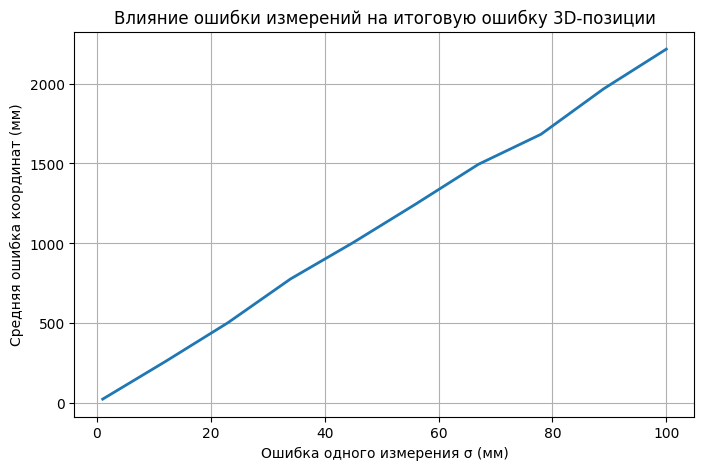
\includegraphics[width=1\textwidth]{error.png} % замените на свой файл
    \caption{график ошибки}
    \label{fig:example}
\end{figure}

Получается что для разрешения координат с погрешностью 30-40 см достаточно иметь дискретизацию по времени 0.1 мс, что достаточно много.


\subsection{Математика}
\subsubsection{Аналитическое решение задачи триангуляции в пространстве по трём расстояниям}

Пусть заданы три опорные точки в плоскости \(z=0\):
\[
P_1 = (x_1, y_1, 0), \qquad
P_2 = (x_2, y_2, 0), \qquad
P_3 = (x_3, y_3, 0),
\]
и измеренные расстояния от неизвестной точки \(P=(x,y,z)\) до них:
\[
r_1,\; r_2,\; r_3.
\]

\subsubsubsection*{1. Уравнения сфер}

Координаты точки \(P\) удовлетворяют системе уравнений трёх сфер:
\[
(x - x_i)^2 + (y - y_i)^2 + z^2 = r_i^2, \qquad i = 1,2,3.
\]

\subsubsubsection*{2. Получение линейной системы для координат \(x\) и \(y\)}

Вычтем уравнения для \(i=2\) и \(i=3\) из уравнения для \(i=1\).  
Так как член \(z^2\) присутствует во всех трёх уравнениях, он сокращается. Получаем:

\begin{align}
2(x_2-x_1)x + 2(y_2-y_1)y &= r_1^2 - r_2^2 + x_2^2 - x_1^2 + y_2^2 - y_1^2, \\
2(x_3-x_1)x + 2(y_3-y_1)y &= r_1^2 - r_3^2 + x_3^2 - x_1^2 + y_3^2 - y_1^2.
\end{align}

В матричной форме:
\[
A
\begin{pmatrix} x \\ y \end{pmatrix}
=
\begin{pmatrix} b_1 \\ b_2 \end{pmatrix},
\]
где
\[
A =
\begin{pmatrix}
2(x_2-x_1) & 2(y_2-y_1) \\
2(x_3-x_1) & 2(y_3-y_1)
\end{pmatrix},
\]
\[
b_1 = r_1^2 - r_2^2 + x_2^2 - x_1^2 + y_2^2 - y_1^2,
\qquad
b_2 = r_1^2 - r_3^2 + x_3^2 - x_1^2 + y_3^2 - y_1^2.
\]

Если опорные точки не коллинеарны, то \(\det A \neq 0\), и система имеет единственное решение:
\[
\begin{pmatrix} x \\ y \end{pmatrix} = A^{-1} \begin{pmatrix} b_1 \\ b_2 \end{pmatrix}.
\]

\subsubsubsection*{3. Определение координаты \(z\)}

После нахождения \(x\) и \(y\) подставим их в первое уравнение сферы:
\[
z^2 = r_1^2 - (x - x_1)^2 - (y - y_1)^2.
\]

Отсюда:
\[
z = \pm\sqrt{\,r_1^2 - (x - x_1)^2 - (y - y_1)^2\,}.
\]

Если
\[
r_1^2 - (x - x_1)^2 - (y - y_1)^2 < 0,
\]
то система не имеет действительных решений (данные несовместны).

Поскольку сферы симметричны относительно плоскости \(z=0\), существует максимум два решения, соответствующие различным знакам корня.  
В данной задаче выбирается решение с положительной высотой:
\[
z > 0.
\]

\subsubsubsection*{4. Итоговое решение}

Искомая точка пересечения сфер:
\[
P = (x, y, z),
\]
где \((x,y)\) находятся из линейной системы
\[
A\begin{pmatrix}x\\y\end{pmatrix} = \begin{pmatrix}b_1\\b_2\end{pmatrix},
\]
а координата \(z\) определяется как
\[
z = \sqrt{\,r_1^2 - (x - x_1)^2 - (y - y_1)^2\,}.
\]

При этом берётся корень со знаком «плюс», так как требуется решение с \(z>0\).

\subsubsection{Решение вычислительными методами}

Для решения данной задачи также можно использовать методы вычислительной математики, например Гаусса Ньютона. Этод метод используется для минимизации суммы квадратов, и имеет оптимальное соотношение точность - скорость.

С учетом выбранного метода, функция для минимизации будет выглядеть следующим образом:

\[
\boxed{%
\; \min_{\mathbf{p}}\; J(\mathbf{p}), \qquad
J(\mathbf{p}) = \sum_{i=1}^{N} w_i\bigl(\,\hat r_i - \|\mathbf{p}-\mathbf{a}_i\|\,\bigr)^2
}
\]

\begin{itemize}
  \item $\hat r_i$ \;— измеренное расстояние от якоря $i$ до объекта .
  \item $\mathbf{a}_i$ \;— вектор координат $i$-го якоря.
  \item $\mathbf{p}$ \;— вектор неизвестных координат объекта.
  \item $w_i$ \;— вес измерения $i$ (обычно обратный дисперсии).
  \item $J(\mathbf{p})$ \;— целевая функция суммы взвешенных квадратов невязок.
\end{itemize}

Описание самого метода приводить не стану. Скажу лишь что для начального приближения имеет смысл брать предыдущую позицию дрона или данные с иннерциальных систем навигации. Тогда метод будет сходиться за считанные итерации и требования к вычислительным мощностям будут минимальны.

\subsubsection{Сравнительный анализ}
Для сравнения точности этих методов предлагаю провести следующий эксперимент:
\\
\\
Смоделируем предполагаемое расположение источников/приемников на платформе.
Рассмотрим конфигурацию из 4 опорных точек, расположенных по углам квадрата с шириной 2 метра.
Аналитический метод предполагает известные расстояния только до трех точек, поэтому мы будем вычилсять координаты для каждой тройки точек в отдельности.

Аналогично поступаем с конфигурацие из 5 точек (такой же квадрат, только дополнительная точка в центре)
\\
\\

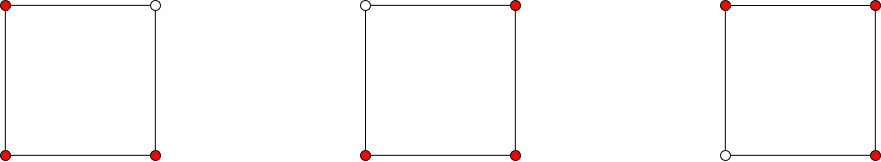
\includegraphics[width=1\textwidth]{Pasted image.png} % замените на свой файл
\begin{center}
    Рис.3 выбор троек точек
\end{center}
Далее полученные координаты усредняем по всем тройкам.
\\
\\
Вычислительный же метод будет заключаться в следующем: в качестве начального прилижение будет браться аналитическое решение по любой из троек, далее будут итерации метода Гаусса-Ньютона, учитывающие расстояние до всех опорных точек.

\subsubsubsection{Измерения}
Будем проводить следующим образом:
\begin{itemize}
    \item Выбираем случайные координаты обьекта, примерно в 20 метрах над платформой
    \item Измеряем расстояния от обьекта до точек
    \item Подмешиваем в расстояния равномерный шум с шириной распределения 20 см
    \item Передаем расстояния в вычислительные методы и получаем результат.
    \item Вычисляем ошибку координат
\end{itemize}
Равномерное распределение ошибки по расстоянию выбрано не случайно, часы могут засечь случайное время в пределах своей разрешающей способности.
\\

Было произмедено 2000 измерений с различными координатами для каждой из конфигураций, получили следующите результаты:
err - расстояние от истинного положения обьекта до вычисленного
srr вычисляется по следующей формуле:
\begin{equation}
SRR = \sum (r_i - R_i)^2
\end{equation}
 где 
 \begin{itemize}
     \item $r_i$ - расстояние от вычисленного положения обьекта до опорной точки
     \item  $R_i$ - расстояние от истинного положения обьекта до опорной точки
 \end{itemize}
\begin{table}[h]
\centering
\caption{4 Sensors}
\begin{tabular}{lcccc}
\toprule
Statistic & analytic err & gn err  & analytic srr  & gn srr \\
\midrule
count & 2000.0000 & 2000.0000 & 2000.0000 & 2000.0000 \\
mean & 0.7494 & 0.7479 & 0.0062 & 0.0032 \\
std & 0.3575 & 0.3587 & 0.0117 & 0.0042 \\
min & 0.0346 & 0.0253 & 4.1826e-10 & 4.1825e-10 \\
25\% & 0.4649 & 0.4627 & 0.0004 & 0.0004 \\
50\% & 0.7349 & 0.7333 & 0.0019 & 0.0016 \\
75\% & 1.0091 & 1.0090 & 0.0063 & 0.0044 \\
max & 1.7822 & 1.7820 & 0.1094 & 0.0287 \\
\bottomrule
\end{tabular}
\end{table}
\begin{table}[h]
\centering
\caption{5 Sensors}
\begin{tabular}{lcccc}
\toprule
Statistic & analytic err & gn err & analytic srr & gn srr \\
\midrule
count & 2000.0000 & 2000.0000 & 2000.0000 & 2000.0000 \\
mean & 0.6755 & 0.7295 & 0.0171 & 0.0067 \\
std & 0.3292 & 0.3615 & 0.0206 & 0.0057 \\
min & 0.0399 & 0.0280 & 0.0001 & 2.0000e-06 \\
25\% & 0.4230 & 0.4511 & 0.0041 & 0.0023 \\
50\% & 0.6519 & 0.7124 & 0.0099 & 0.0053 \\
75\% & 0.9082 & 0.9931 & 0.0220 & 0.0096 \\
max & 1.7357 & 1.8415 & 0.2038 & 0.0393 \\
\bottomrule
\end{tabular}
\end{table}
\\

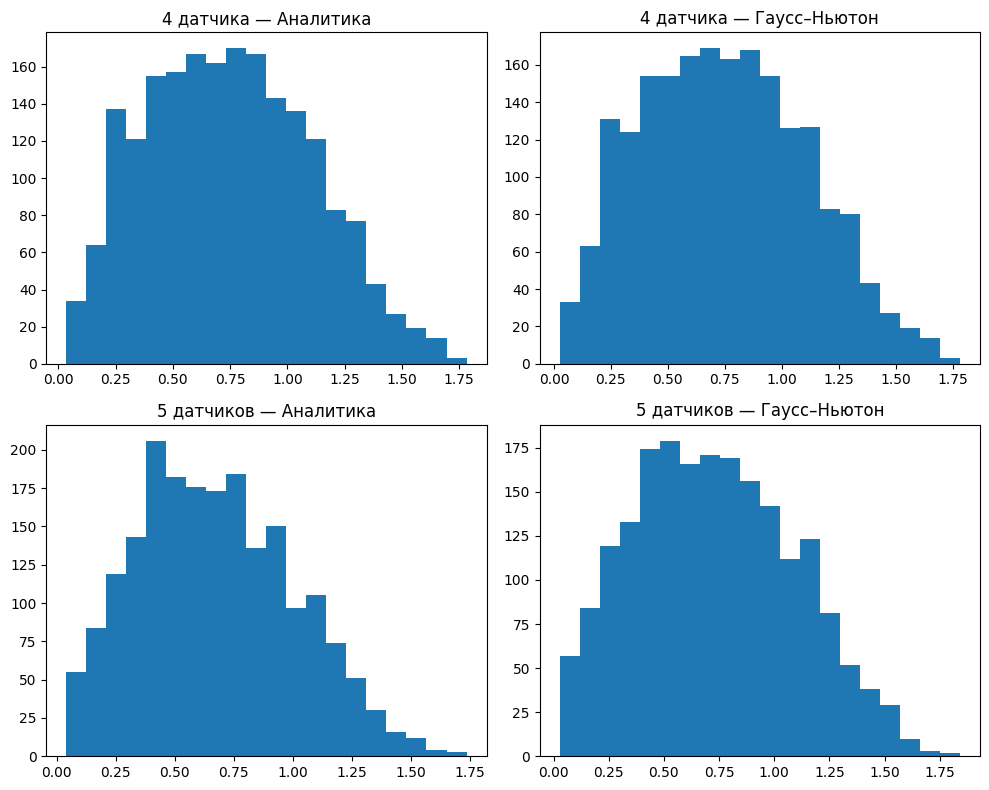
\includegraphics[width=1\textwidth]{method_err.png} % замените на свой файл

Как видно из результатов аналитический метод дает меньшую ошибку по координатам, тогда как ГН имеет меньше SRR (что неудивительно, ведь ГН построен на этой величине). Нас интересуют точные координаты, поэтому выбираем аналитический метод, тем более, он дешевле вычислительно.
\\

Я эксперементировал с улучшениями ГН и другими вычислительными методами, но мне не удалось превзойти результаты аналитического метода. Возможно методы машинного обучения могут это сделать.
\\

Как видно из результатов, увеличение количества точек не сильно повышают точность, возможно дело в плохом их расположении.
\section{Реализация}

\subsection{Конфигурация}

Имеет смысл рассматривать две возможные конфигурации:

\begin{enumerate}
  \item 4 излучателя на платформе, 1 приемник на дроне
  \item 4 приемника на платформе, 1 излучатель на дроне
\end{enumerate}
Я больше склоняюсь к первому варианту, так как:

\begin{itemize}
  \item не будет ограничений на мощность излучателей (мощные излучатели могут весить довольно много)
  \item дрон будет первым узнавать о своей позиции (ему нужнее)
\end{itemize}
Единственное что может вызвать проблему это усилители и фильтры для приемника, но они не должны весить много.

\subsection{Синхронизация}

Для корректного вычисления расстояния необходимо чтобы часы излучатеолей и приемника были синхронизованы. 

Существует несколько решений этой проблемы:

\begin{itemize}
  \item В случае привязного дрона проблема решается легко: по кабелю будет идти синхронизующий сигнал.
  \item Радиосвязь между системами излучателей и приемника.
  \item Синхронизовать часы до запуска, этого должно хватить на несколько часов полета.
\end{itemize}
Конкретное решение выбирается по обстоятельствам.

\subsection{Конструкция}
На подвижной платформе располагаются 4 излучателя в четко заданных позиция на максимальном расстоянии друг от друга. К корпусу платформы жестко закрепляется акселерометр, для отслеживания наклона платформы относительно горизонта.
\vspace{5mm}

Обновление позиции можно будет проводить достаточно часто, особенно при использовании совместно с инерциальными системами навигации.
\vspace{5mm}

Для упрощения предлагаю обновлять позицию 2 раза в секунду.
Кождому излучателю необходимо будет отправлять импульс раз в 0.5 сек. Для того чтобы отличать сигнал от разных излучателей необходимо разделить их импульсы временем $> \Delta t$

\begin{equation}
 \Delta t = \frac{\Delta l}{c}
\end{equation}

где:
\begin{itemize}
    \item $\Delta l$ - максимальное расстояние между излучателями
    \item $c$ - скорость звука
\end{itemize}

Тогда мы можем быть точно уверены, что первый принятый сигнал - это первый отправленный, и т. д.

На дроне устанавливается приемник, направленный вниз, и находящийся в области прямой видимости излучателей. Также устанавливается усилитель и фильтр сигнала. Важно добиться высокого соотношения сигнал/шум, это напрямую влияет на максимальное расстояние навигации.

Еще еобходимо будет установить микроконтроллер, который будет заниматься засеканием времени и вычислениями, но требования к нему довольно низкие.

\cite{vishn2020}

\end{document}
